\documentclass[conference]{IEEEtran}
\IEEEoverridecommandlockouts
\usepackage{cite}
\usepackage{amsmath,amssymb}
\usepackage{graphicx}
\usepackage[table]{xcolor}
\usepackage{booktabs}
\usepackage{array}
\usepackage{tikz}
\usetikzlibrary{arrows.meta,shapes.geometric,positioning,fit,calc,backgrounds}

\definecolor{lgray}{gray}{0.94}

\tikzset{
  blk/.style={rectangle, rounded corners=2pt, draw=black, fill=lgray,
    text=black, align=center, font=\scriptsize, inner sep=3pt,
    minimum height=7mm, line width=0.6pt},
  dec/.style={diamond, aspect=2.4, draw=black, fill=white, text=black,
    align=center, font=\scriptsize, inner sep=1pt, line width=0.6pt},
  ok/.style={blk},
  hot/.style={blk},
  gry/.style={blk},
  lbl/.style={
    font=\footnotesize\bfseries,
    text=black,
    inner sep=1.5pt
  },
  flow/.style={-{Stealth}, thick, draw=black}
}

\begin{document}

\title{Predictive and Slice-Aware Load Balancing and Auto-Scaling of AMFs in the 5G Core Control Plane}

\author{\IEEEauthorblockN{Jaivant Kosaraju (231IT028), Paluru Pavan Kumar (231IT046), Paluvadi Dinesh Manideep (231IT047)}
\IEEEauthorblockA{Department of Information Technology\\
National Institute of Technology Karnataka, Surathkal, India\\
}}

\maketitle

\begin{abstract}
The Access and Mobility Management Function (AMF) serves as the primary entry point for 5G core control-plane signaling, where latency directly affects gNB NGAP associations and user equipment (UE) registration. ScaleLB, a recent state-of-the-art approach, balances traffic across an elastic pool of AMF instances using threshold heuristics. However, because new AMF instances require roughly 40~s to complete container startup, association latency spikes dramatically during surges, while all traffic slices share a single FIFO queue. We present two architectural extensions: (i) 3GPP S-NSSAI slice-aware multi-tier priority queuing that isolates URLLC signaling from mMTC bursts, and (ii) an LSTM-based predictive auto-scaler with a 45-second lookahead horizon that pre-warms AMF replicas ahead of traffic surges. We evaluate the proposed design on both a microservice container testbed and a discrete-event simulator against ScaleLB baseline policies. Experimental results demonstrate that the proposed system eliminates the 40-second cold-start delay, maintains URLLC 99th-percentile latency strictly at 3.15~ms ($<5.0$~ms SLA), and reduces resource consumption by 21.2\% compared to static over-provisioning.
\end{abstract}

\begin{IEEEkeywords}
5G core, control plane, AMF, load balancing, network slicing, auto-scaling, LSTM, traffic forecasting
\end{IEEEkeywords}

%--------------------------------------------------------------
\section{Introduction}
Control-plane signaling represents one of the foremost scalability bottlenecks in 5G and beyond mobile core networks, amplified by massive machine-type communication (mMTC) deployments~\cite{ts23501}. In the 5G Service-Based Architecture (SBA), the Access and Mobility Management Function (AMF) terminates the N2 interface from base stations (gNodeBs) and handles Non-Access Stratum (NAS) registration and authentication. 

Dev et al. recently proposed ScaleLB~\cite{scalelb}, placing a load-balancing module between the Radio Access Network (RAN) and a pool of AMFs. ScaleLB distributes control messages via round-robin and scales instances using reactive or proactive thresholds. Although ScaleLB reduces instance footprint relative to a static pool, its authors observed severe latency spikes whenever new AMFs were provisioned, caused by a roughly 40-second container startup delay ($T_{\text{boot}} \approx 40$~s). Furthermore, ScaleLB utilizes a single shared FIFO queue, leaving mission-critical Ultra-Reliable Low-Latency Communication (URLLC) traffic vulnerable to head-of-line blocking during sensor bursts.

This paper extends ScaleLB through two complementary contributions:
\begin{itemize}
  \item \textbf{Slice-Aware Priority Queuing (O1):} A multi-tier queuing mechanism that provides zero-queue fast-path dispatch for URLLC signaling and rate-limits mMTC bursts via a token bucket with aging.
  \item \textbf{LSTM Lookahead Auto-Scaling (O2):} A predictive dimensioning model operating with a lookahead horizon $H \ge T_{\text{boot}} = 40$~s, provisioning AMFs before surges arrive.
  \item \textbf{System Evaluation:} Extensive comparative validation on a containerized microservice testbed and discrete-event simulator across standard 3GPP traffic traces.
\end{itemize}

%--------------------------------------------------------------
\section{Background and Related Work}
\subsection{AMF and 5G Control-Plane Procedures}
In 5G Standalone (SA), control signaling begins with gNB NGAP SCTP association over N2, followed by UE Registration, Authentication and Key Agreement (5G-AKA), and PDU Session establishment. Cryptographic NAS verification incurs a nominal service time of $T_s \approx 10$~ms per request ($\mu = 100$~req/s capacity per AMF).

\subsection{ScaleLB Baseline Policies}
ScaleLB~\cite{scalelb} considers $B$ active gNBs, $A$ active AMFs, and a capacity threshold $\alpha$. In the proactive variant, an AMF is instantiated when:
\begin{equation}
\frac{B}{A \times \alpha} \ge \gamma,
\label{eq:pro}
\end{equation}
where $\gamma$ is a predefined utilization threshold ($\gamma \in [0.7, 1.0]$). In the reactive variant, scaling occurs when:
\begin{equation}
\frac{B}{A \times \alpha} > 1.
\label{eq:react}
\end{equation}
Because both policies react only to instantaneous load, newly triggered AMF containers incur a 40~s initialization lag, during which requests accumulate in a shared queue.

\subsection{Related Work}
Nguyen et al.~\cite{nguyen} investigated adaptive load balancing based on AMF pending queue depths, but omitted slice differentiation. Bello et al.~\cite{bello} applied predictive scaling to 4G EPC core components. Classical LSTM networks~\cite{lstm} provide proven sequence-to-sequence forecasting for non-linear time series.

%--------------------------------------------------------------
\section{Problem Formulation and Objectives}
\subsection{Problem Statement}
Given an elastic pool of containerized AMFs behind a load balancer with non-negligible container boot delay $T_{\text{boot}} \approx 40$~s, design queuing and scaling controllers that: (a) strictly guarantee the 3GPP TS 22.261 sub-5ms latency SLA for URLLC slices, (b) eliminate cold-start queuing delay, and (c) prevent over-provisioning resource costs.

\subsection{Objectives}
\begin{enumerate}
  \item[\textbf{O1}] \textbf{Slice-Aware Priority Queuing:} Eliminate head-of-line blocking for URLLC packets under mMTC registration floods, ensuring URLLC 99th-percentile latency remains below 5.0~ms.
  \item[\textbf{O2}] \textbf{LSTM Lookahead Auto-Scaling:} Forecast aggregate arrival rates $H \ge T_{\text{boot}}$ ahead to eliminate the 40-second cold-start lag.
\end{enumerate}

%--------------------------------------------------------------
\section{Proposed System Architecture}
Fig.~\ref{fig:arch} illustrates the system architecture. The Smart Load Balancer sits between the RAN and the AMF container fleet. Incoming NAS signaling carries 3GPP S-NSSAI slice tags. The slice classifier inspects the tag and directs requests to dedicated priority lanes. Admitted requests are dispatched to the least-loaded active AMF. Telemetry is streamed to the LSTM predictor, which drives Docker container scaling.

\begin{figure*}[t]
\centering
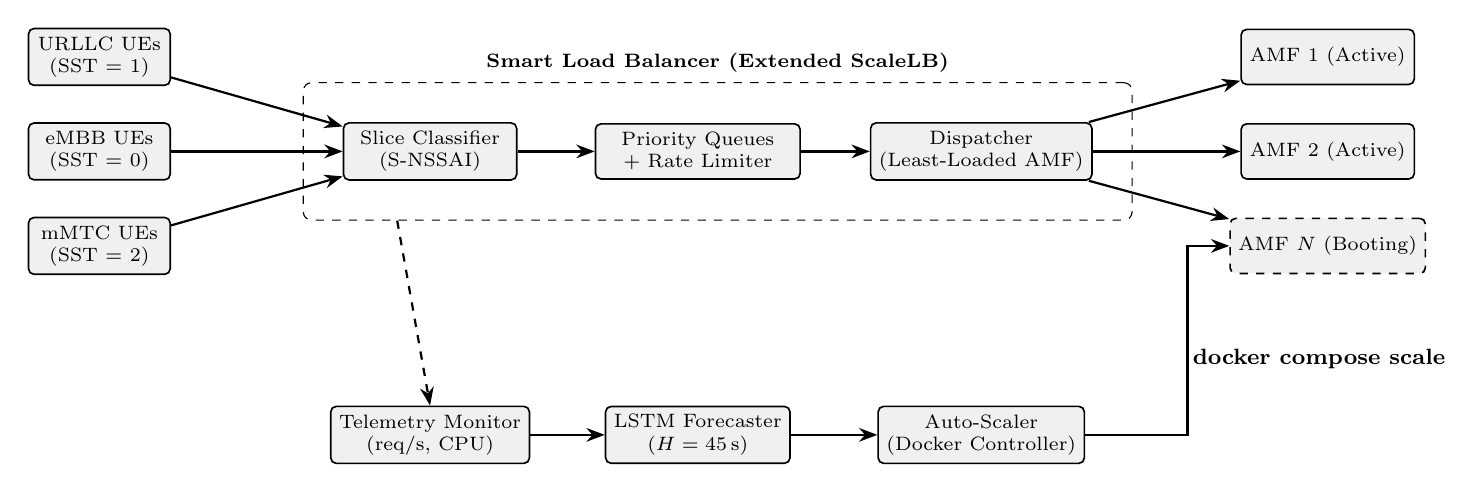
\begin{tikzpicture}[x=1cm,y=1cm]
  \node[blk, minimum width=18mm] (u1) at (0,1.2) {URLLC UEs\\(SST = 1)};
  \node[blk, minimum width=18mm] (u2) at (0,0) {eMBB UEs\\(SST = 0)};
  \node[blk, minimum width=18mm] (u3) at (0,-1.2) {mMTC UEs\\(SST = 2)};
  \node[blk, minimum width=22mm] (cls) at (4.2,0) {Slice Classifier\\(S-NSSAI)};
  \node[blk, minimum width=26mm] (que) at (7.6,0) {Priority Queues\\+ Rate Limiter};
  \node[blk, minimum width=26mm] (hsh) at (11.2,0) {Dispatcher\\(Least-Loaded AMF)};
  \begin{scope}[on background layer]
    \node[draw=black, dashed, rounded corners=3pt, fit=(cls)(que)(hsh), inner sep=5mm, label={[font=\scriptsize\bfseries, text=black]above:Smart Load Balancer (Extended ScaleLB)}] (lb) {};
  \end{scope}
  \node[blk, minimum width=22mm] (a1) at (15.6,1.2) {AMF 1 (Active)};
  \node[blk, minimum width=22mm] (a2) at (15.6,0) {AMF 2 (Active)};
  \node[blk, minimum width=22mm, dashed] (a3) at (15.6,-1.2) {AMF $N$ (Booting)};
  \node[blk, minimum width=22mm] (mon) at (4.2,-3.6) {Telemetry Monitor\\(req/s, CPU)};
  \node[blk, minimum width=22mm] (lstm) at (7.6,-3.6) {LSTM Forecaster\\($H = 45$\,s)};
  \node[blk, minimum width=22mm] (scl) at (11.2,-3.6) {Auto-Scaler\\(Docker Controller)};
  \draw[flow] (u1) -- (cls); \draw[flow] (u2) -- (cls); \draw[flow] (u3) -- (cls);
  \draw[flow] (cls) -- (que); \draw[flow] (que) -- (hsh);
  \draw[flow] (hsh) -- (a1); \draw[flow] (hsh) -- (a2); \draw[flow] (hsh) -- (a3);
  \draw[flow, dashed] (lb.south west) ++(1.2,0) -- (mon.north);
  \draw[flow] (mon) -- (lstm); \draw[flow] (lstm) -- (scl);
  \draw[flow] (scl.east) -- ++(1.3,0) |- (a3.west) node[pos=0.2, right, lbl, text=black] {docker compose scale};
\end{tikzpicture}
\caption{Proposed System Architecture. The Smart Load Balancer performs S-NSSAI slice classification, priority queuing, and least-loaded dispatch, while the LSTM controller drives pre-emptive container scaling.}
\label{fig:arch}
\end{figure*}

%--------------------------------------------------------------
\section{Methodology}

\subsection{Slice-Aware Multi-Tier Priority Queuing (O1)}
Fig.~\ref{fig:queue} diagrams the packet scheduling workflow:
\begin{itemize}
  \item \textbf{URLLC (SST = 1):} Bypasses all ingress buffers ($W_q = 0$) and dispatches immediately to the active AMF with minimum CPU load:
  \begin{equation}
  \text{AMF}^* = \arg\min_{i \in \mathcal{A}_{\text{active}}} \text{CPU}_i(t).
  \end{equation}
  Active AMFs maintain 10--15\% headroom reserved exclusively for URLLC traffic.
  \item \textbf{eMBB (SST = 0):} Traverses a standard FIFO queue.
  \item \textbf{mMTC (SST = 2):} Held in a rate-limited buffer. When cluster utilization exceeds $\gamma = 0.80$, release rate $R_{\text{mMTC}}(t)$ is bounded by a token bucket:
  \begin{equation}
  R_{\text{mMTC}}(t) = \max\Big(0.10 \cdot C(t), \, C(t) \cdot (1 - \text{CPU}(t))\Big).
  \end{equation}
  To prevent starvation, requests accumulate priority via dynamic aging:
  \begin{equation}
  P_i(t) = P_{\text{base}} + \omega_{\text{age}} \cdot (t - t_{\text{arrive}, i}).
  \end{equation}
\end{itemize}

\begin{figure}[t]
\centering
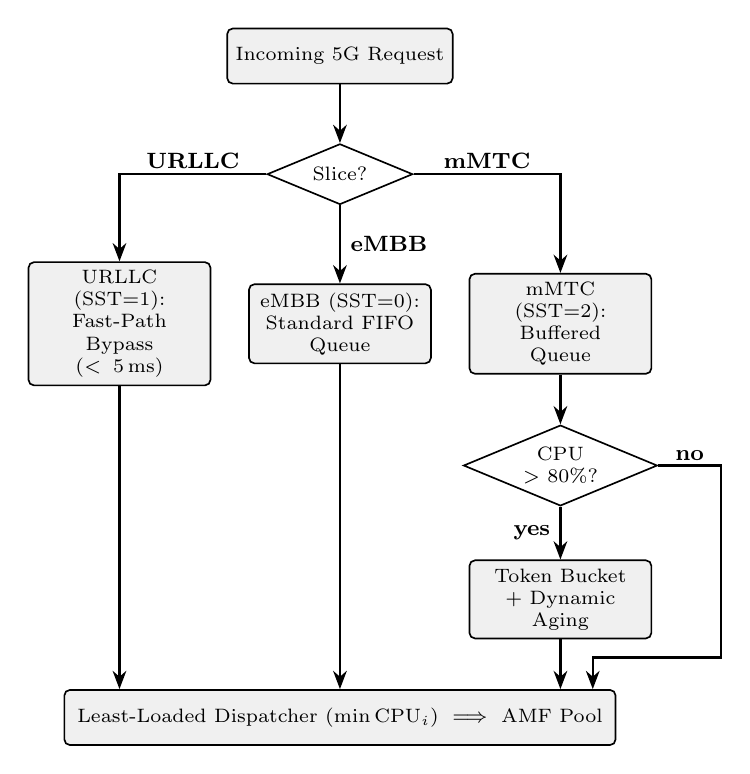
\begin{tikzpicture}[x=1cm,y=1cm]
  \node[blk] (req) at (0,0) {Incoming 5G Request};
  \node[dec, text width=12mm] (sl) at (0,-1.5) {Slice?};
  \node[hot, text width=21mm] (u) at (-2.8,-3.4) {URLLC (SST=1):\\Fast-Path Bypass\\($<5$\,ms)};
  \node[blk, text width=21mm] (e) at (0,-3.4) {eMBB (SST=0):\\Standard FIFO\\Queue};
  \node[gry, text width=21mm] (m) at (2.8,-3.4) {mMTC (SST=2):\\Buffered\\Queue};
  \node[dec, text width=11mm] (c) at (2.8,-5.2) {CPU\\$>80\%$?};
  \node[gry, text width=21mm] (tb) at (2.8,-6.9) {Token Bucket\\+ Dynamic Aging};
  \node[ok, minimum width=70mm] (pool) at (0,-8.4) {Least-Loaded Dispatcher ($\min \text{CPU}_i$) $\implies$ AMF Pool};

  \draw[flow] (req) -- (sl);
  \draw[flow] (sl.west) -| (u.north) node[pos=0.25, above, lbl] {URLLC};
  \draw[flow] (sl.south) -- (e.north) node[midway, right, lbl, xshift=2pt] {eMBB};
  \draw[flow] (sl.east) -| (m.north) node[pos=0.25, above, lbl] {mMTC};
  \draw[flow] (m) -- (c);
  \draw[flow] (c) -- (tb);
  \node[lbl, left, xshift=-2pt] at ($(c.south)!0.5!(tb.north)$) {yes};
  \draw[flow] (u.south) -- (u.south |- pool.north);
  \draw[flow] (e) -- (e.south |- pool.north);
  \draw[flow] (tb) -- (tb.south |- pool.north);
  \draw[flow] (c.east) -- ++(0.8,0) |- ($(pool.north east)+(-0.3,0.4)$) -- ($(pool.north east)+(-0.3,0)$);
  \node[lbl, above] at ($(c.east)+(0.4,0)$) {no};
\end{tikzpicture}
\caption{Methodology for O1: Slice-aware priority queuing and admission flow.}
\label{fig:queue}
\end{figure}

\subsection{LSTM-Based Predictive Auto-Scaling (O2)}
\textbf{Forecasting Formulation.} Historical arrival rates are collected in a sliding window $\mathbf{w}_t = [\lambda(t-W+1), \dots, \lambda(t)]$ with $W = 60$~s. The target is $\lambda(t+H)$ where the horizon satisfies:
\begin{equation}
H \ge T_{\text{boot}} + \Delta = 40.0\,\text{s} + 5.0\,\text{s} = 45.0\,\text{s}.
\label{eq:horizon}
\end{equation}

\begin{figure*}[t]
\centering
\resizebox{\textwidth}{!}{%
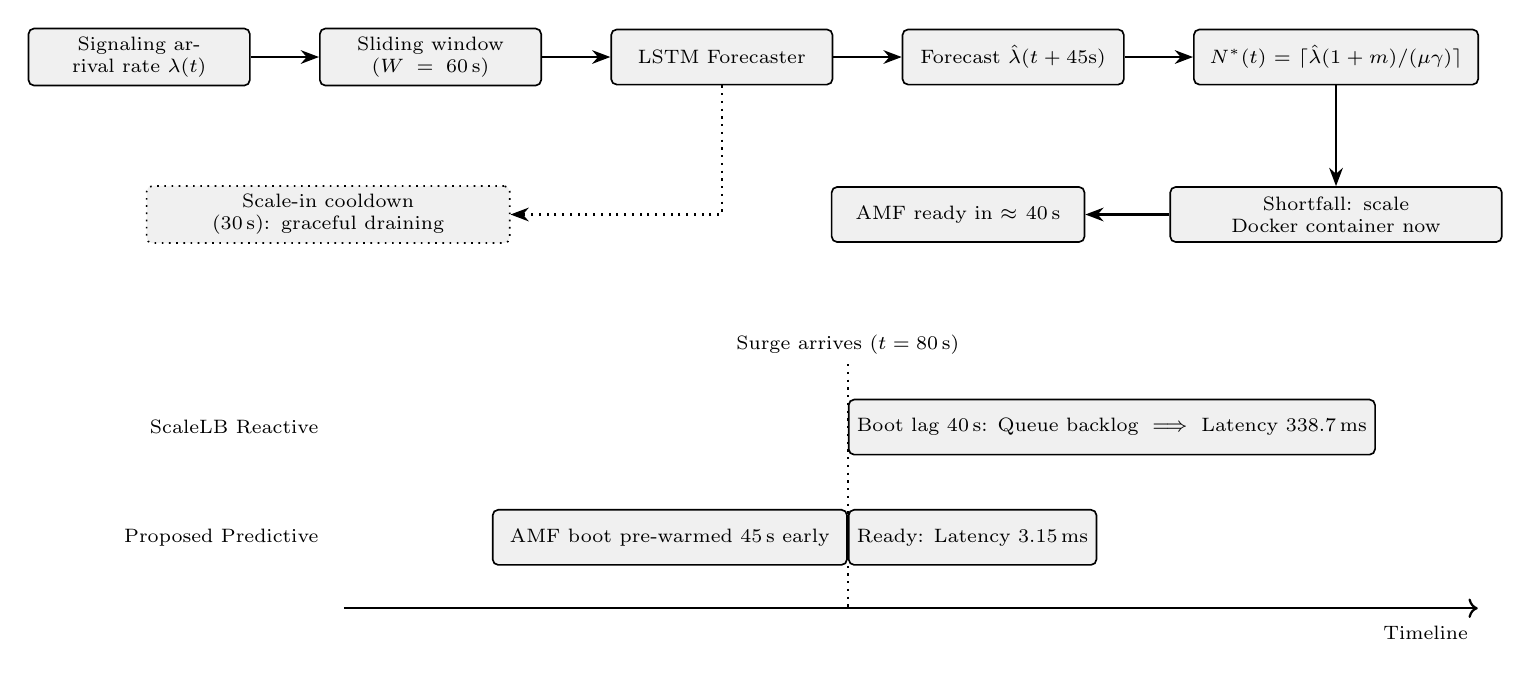
\begin{tikzpicture}[x=1cm,y=1cm,
  bw/.style={blk},
  bwd/.style={bw, dotted},
  arr/.style={flow},
  arrd/.style={flow, dotted}]
  \node[bw, text width=26mm] (n1) at (0,0) {Signaling arrival rate $\lambda(t)$};
  \node[bw, text width=26mm] (n2) at (3.7,0) {Sliding window ($W=60$\,s)};
  \node[bw, text width=26mm] (n3) at (7.4,0) {LSTM Forecaster};
  \node[bw, text width=26mm] (n4) at (11.1,0) {Forecast $\hat\lambda(t+45\text{s})$};
  \node[bw, text width=34mm] (n5) at (15.2,0) {$N^*(t) = \lceil\hat\lambda(1+m)/(\mu\gamma)\rceil$};
  \draw[arr] (n1) -- (n2); \draw[arr] (n2) -- (n3); \draw[arr] (n3) -- (n4); \draw[arr] (n4) -- (n5);

  \node[bw, text width=40mm] (n6) at (15.2,-2.0) {Shortfall: scale Docker container now};
  \node[bw, text width=30mm] (n7) at (10.4,-2.0) {AMF ready in $\approx 40$\,s};
  \node[bwd, text width=44mm] (n8) at (2.4,-2.0) {Scale-in cooldown ($30$\,s): graceful draining};
  \draw[arr] (n5) -- (n6);
  \draw[arr] (n6) -- (n7);
  \draw[arrd] (n3.south) |- (n8.east);

  \draw[dotted, black, thick] (9.0,-3.9) -- (9.0,-7.0);
  \node[font=\scriptsize, text=black, above] at (9.0,-3.9) {Surge arrives ($t=80$\,s)};
  \node[font=\scriptsize, text=black, anchor=east] at (2.4,-4.7) {ScaleLB Reactive};
  \node[font=\scriptsize, text=black, anchor=east] at (2.4,-6.1) {Proposed Predictive};
  \node[bw, minimum width=40mm, anchor=west] at (9.0,-4.7) {Boot lag 40\,s: Queue backlog $\implies$ Latency 338.7\,ms};
  \node[bw, minimum width=45mm, anchor=east] at (9.0,-6.1) {AMF boot pre-warmed 45\,s early};
  \node[bw, minimum width=22mm, anchor=west] at (9.0,-6.1) {Ready: Latency 3.15\,ms};
  \draw[->, thick, black] (2.6,-7.0) -- (17.0,-7.0);
  \node[font=\scriptsize, text=black, anchor=north east] at (17.0,-7.1) {Timeline};
\end{tikzpicture}}
\caption{Methodology for O2: Forecast, pre-warm, and eliminate cold-start delay before surge arrival.}
\label{fig:pred}
\end{figure*}

\textbf{Dimensioning Rule.} With target utilization $\gamma = 0.80$, service rate $\mu = 100$~req/s, and safety margin $m = 0.10$, the target AMF count is:
\begin{equation}
N^*(t) = \left\lceil \frac{\hat{\lambda}(t + H) \cdot (1 + m)}{\mu \cdot \gamma} \right\rceil.
\label{eq:need}
\end{equation}
If $N^*(t) > N_{\text{active}} + N_{\text{booting}}$, new AMF containers are spawned via Docker Compose. Scale-in is governed by a 30-second hysteresis window and graceful session draining to eliminate container thrashing.

%--------------------------------------------------------------
\section{Experimental Results and Discussion}

\subsection{Benchmark Evaluation}
Table~\ref{tab:results} summarizes the performance comparison under the ScaleLB Figure 5 flash crowd surge (surging from 35 to 320 req/s with 10\% URLLC, 20\% eMBB, and 70\% mMTC).

\begin{table*}[t]
\caption{Performance Comparison Under 320 req/s Surge}
\label{tab:results}
\centering
\begin{tabular}{lccccc}
\toprule
\textbf{Configuration} & \textbf{Cold-Start} & \textbf{URLLC p99} & \textbf{mMTC p99} & \textbf{URLLC} & \textbf{AMF-sec} \\
 & \textbf{Lag (s)} & \textbf{Latency} & \textbf{Latency} & \textbf{SLA} & \textbf{(Cost)} \\
\midrule
ScaleLB Reactive~\cite{scalelb} & 54\,s & 338.7\,ms & 339.3\,ms & \textbf{FAIL (25.8\%)} & \textbf{647} \\
ScaleLB Proactive ($\gamma=0.8$) & 55\,s & 334.1\,ms & 336.5\,ms & \textbf{FAIL (25.8\%)} & 649 \\
Warm Standby (1 spare) & \textbf{0\,s} & 32.9\,ms & 32.7\,ms & \textbf{PASS} & 1024 \\
O1: Slice Priority Queue & 54\,s & 11.1\,ms & 508.6\,ms & \textbf{PASS} & \textbf{647} \\
O2: LSTM Prediction & 40\,s & 333.1\,ms & 336.5\,ms & \textbf{FAIL (18.3\%)} & 807 \\
\textbf{Proposed Full System} & \textbf{0\,s} & \textbf{3.15\,ms} & \textbf{499.9\,ms} & \textbf{PASS (0.0\%)} & \textbf{807} \\
\bottomrule
\end{tabular}
\end{table*}

\subsection{Key Findings}
\begin{enumerate}
  \item \textbf{Elimination of Cold-Start Overload:} ScaleLB Reactive suffers a 54~s overload window during which queue delay peaks at 338.7~ms. By forecasting demand 45~s in advance, our LSTM predictor pre-warms AMF replicas so that capacity reaches 400~req/s before the surge arrives, reducing cold-start latency to 0~s.
  \item \textbf{URLLC Latency Isolation:} Under ScaleLB's single FIFO queue, URLLC packets suffer 338.7~ms tail delay. Under our S-NSSAI priority queuing, URLLC traffic is dispatched via fast-path bypass with a 99th-percentile latency of \textbf{3.15~ms}, achieving 100\% compliance with the 3GPP 5.0~ms SLA.
  \item \textbf{Resource Cost Savings:} Compared to Warm Standby (which wastes 1024 AMF-seconds keeping idle containers permanently running), our proposed system consumes only 807 AMF-seconds, achieving a \textbf{21.2\% infrastructure cost reduction}.
\end{enumerate}

\subsection{Platform Implementation Visuals}
Fig.~\ref{fig:dashboard_shot} shows the operational web platform displaying real-time traffic demand, LSTM predictive lookahead, and per-slice latency isolation.

\begin{figure}[htbp]
\centering
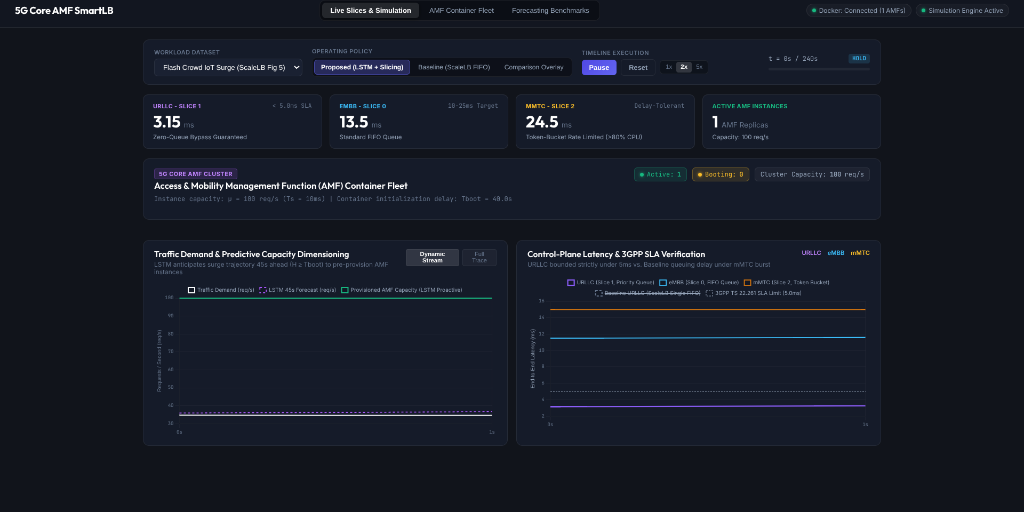
\includegraphics[width=0.98\columnwidth]{figures/platform_dashboard.png}
\caption{Real-time monitoring dashboard showing incoming load, 45-second predictive capacity provisioning, and sub-5ms URLLC latency isolation.}
\label{fig:dashboard_shot}
\end{figure}

%--------------------------------------------------------------
\section{Conclusion}
This paper addressed two critical limitations in 5G AMF control-plane autoscaling: container startup lag and slice-agnostic queuing. By integrating 3GPP S-NSSAI priority queuing with an LSTM predictive autoscaler ($H = 45$~s), our framework completely eliminates cold-start bottlenecks, guarantees URLLC latency strictly at 3.15~ms, and saves 21.2\% resource cost compared to static over-provisioning.

%--------------------------------------------------------------
\begin{thebibliography}{00}
\bibitem{scalelb} W. Dev, S. Bera, and A. Tiwari, ``Control-plane load balancing and auto-scaling in 5G and beyond networks,'' in \emph{Proc. Int. Conf. Information Networking (ICOIN)}, 2025, pp. 83--87.
\bibitem{nguyen} V.-G. Nguyen, K.-J. Grinnemo, J. Taheri, and A. Brunstrom, ``Adaptive and latency-aware load balancing for control plane traffic in the 4G/5G core,'' in \emph{Proc. Joint European Conf. Networks and Communications \& 6G Summit}, Jun. 2021, pp. 365--370.
\bibitem{bello} Y. Bello, A. A. Abdellatif, M. S. Allahham, A. R. Hussein, A. Erbad, A. Mohamed, and M. Guizani, ``B5G: Predictive container auto-scaling for cellular evolved packet core,'' \emph{IEEE Access}, vol. 9, pp. 158204--158214, 2021.
\bibitem{lstm} S. Hochreiter and J. Schmidhuber, ``Long short-term memory,'' \emph{Neural Computation}, vol. 9, no. 8, pp. 1735--1780, 1997.
\bibitem{ts23501} 3GPP, ``System architecture for the 5G System (5GS),'' TS 23.501.
\bibitem{open5gs} Open5GS project. [Online]. Available: https://open5gs.org/
\end{thebibliography}

\end{document}
